\chapter{Testumgebung}

\section{Einführung}

Die Testumgebung setzt sich aus einer aufgesetzten KVM Umgebung zusammen, auf 
welche via SSH verbunden wird, um neue Services abonnieren zu können und die 
nötigen Ressourcen zu allozieren.

\section{KVM/QEMU}

In Unserer Umgebung wurde KVM standardmässig aufgesetzt und zusätzlich der 
libvirtd Service installiert, welcher das erstellen, ändern und löschen von 
Ressourcen erlaubt.

\section{Aufbau}

In unserer Testumgebung wurde die SDDC Software und KVM auf jeweils einem eigenen Server betrieben.
Zwischen den Systemen wird mit SSH kommuniziert.
\begin{center}
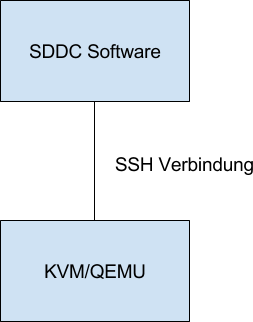
\includegraphics[width=0.33\textwidth]{./12_Appendix/images/kvm}
\end{center}

\section{Spezifikationen KVM Server}

\textbf{vCPUs:} 4
\textbf{RAM:} 4 GB
\textbf{Hauptspeicher:} 20 GB

\section{Spezifikationen SDDC Server}

\textbf{vCPUs:} 2
\textbf{RAM:} 2 GB
\textbf{Hauptspeicher:} 20 GB